\documentclass[letterpaper,twocolumn,10pt]{article}
\usepackage{usenix,epsfig,authblk}
\usepackage{xcolor}
\usepackage{hyperref}
\usepackage{graphicx}

\newcommand{\pname}{Resourceful}
\newcommand{\lnote}[1]{\textcolor{red}{[\textit{#1}]}} %notes
\newcommand*\aorder[1][\value{footnote}]{\footnotemark[#1]}
\renewcommand\Authsep{\hskip 1cm}
\renewcommand\Authands{\hskip 1cm}

\begin{document}

%don't want date printed
\date{}

%make title bold and 14 pt font (Latex default is non-bold, 16 pt)
\title{\Large \bf \pname: Fine-grained Resource Accounting}

%for single author (just remove % characters)
\author{Lucian Carata\thanks{in alphabetical order}\aorder}
\author{Oliver Chick\aorder}
\author{James Snee\aorder}
\author{\authorcr{}Ripduman Sohan}
\author{Andrew Rice}
\author{Andy Hopper}
\affil{Computer Laboratory, University of Cambridge, UK\\
       \texttt{\{firstname.lastname\}@cl.cam.ac.uk}}

\maketitle

% Use the following at camera-ready time to suppress page numbers.
% Comment it out when you first submit the paper for review.
\thispagestyle{empty}


\subsection*{Abstract}
We outline the design and prototype implementation of \pname, a tool that allows fine-grained (system call level) resource accounting for the Linux kernel. The system can account for both synchronous and asynchronous CPU, memory and IO costs of given application calls, while incurring a low overhead. \lnote{to be completed...}

\section{Introduction}
%TODO(lc525): modify in accordance to Andy's comments
Any system experiencing high contention on particular resources will show more variability in its behavior, becoming less predictable in terms of performance and failure rates \cite{?}. This is why resource consumption metrics like CPU, memory or IO are often used as a proxy for system behavior and health, in both human-driven and automated processes (e.g. by an engineer evaluating increased tail latency causes or a distributed scheduler making decisions about task migration).

However, low resource usage is not desirable, either: there has been a constant push for increasing server utilization and reducing running costs in modern datacenters. Those are typically achieved through service aggregation, where multiplexing several applications on a single physical host is done either through hypervisor-based virtualization (VM's), lightweight virtualization (containers), or by running multiple services on the same OS, depending on the required level of isolation, SLAs, etc. 
%\lnote{In order to lower overheads, it seems likely that lighter-weight OS-based virtualization solutions such as containers will become more common.}
Here, the entities managing hardware resources (the hypervisor and/or the OS kernel) are by design seen as black boxes by any process executing on top. This makes it difficult to assess any side effects that a running process might have upon other processes sharing the same resources. Those side effects could manifest as performance degradation (for example, in cache trashing and IO storms) or changes in the output of the system (fewer results returned, loss of precision if running timeout-based processing algorithms).

As more services will start sharing the same hardware resources, the importance of measuring and understanding both the causes and consequences of such variations in the properties of the system will increase. This justifies the need for gathering accurate resource accounting data \lnote{at the hypervisor/kernel level?}.

It is of course possible to coarsely measure variation in terms of \textit{aggregate} resource consumption using existing profiling and monitoring tools. Linux kernels provide mechanisms such as the \texttt{getrusage()} call (small number of fixed statistics), \texttt{perf} (for reading performance counters), and \texttt{ftrace}. Specialized tools such as \texttt{iotop} or \texttt{netstat} use information exposed through the \texttt{$\backslash$proc} virtual filesystem, while more general-purpose tools like SystemTap allow the user to write scripts that can gather similar data. However, we make the observation that those, by themselves, fall short in the following important dimensions: 

(i) \textbf{Accounting granularity and aggregation:} most of the mechanisms above can only obtain system-wide or per-process statistics. Because the data comes pre-aggregated, it is difficult to understand the contribution of a particular process \textit{activity} (i.e. a system call or set of application function calls) towards the total resource consumption. For example, if a one tries to look at how resource utilization varies for a server process between low-latency and high-latency responses (in order to infer causes and make optimizations), it will not be able to do so based on per-process or even per-thread aggregated data. Instead, fine-grained information is needed: in our example, per system call data aggregated over the lifetime of the request-response cycle. This type of accounting is often avoided because of the overhead introduced by existing tools (such as ftrace) when dealing with per-function tracing.

(ii) \textbf{Accounting for resources consumed asynchronously:} not all the effects of a given call occur during its execution. However, there are no existing tools for linking asynchronous kernel tasks (together with the resources that they consume) to the application actions that triggered their execution. A very simple example here is a process writing data to disk: while the application makes multiple calls to \texttt{write(...)} on a particular file descriptor, there might be no immediate IO activity on disk because the kernel uses a buffer cache. The actual disk IO will occur asynchronously (dependent on the IO scheduler, the expiration of a default flushing interval, an explicit call to \texttt{fsync}, etc). Simply recording some resource consumption metrics before and after a \texttt{write(...)} call would not produce accurate results. The linux kernel has multiple ways of executing such asynchronous tasks (timers, tasklets, workqueues, software interrupts), and understanding when they run because of particular application actions is important in explaining shared resource usage.

(iii) \textbf{Online analysis and feedback:} with the exception of \texttt{getrusage()}, most kernel-level resource accounting mechanisms available are designed for debugging or offline analysis scenarios --- the monitored processes have no control over what is being recorded and how, and the final output is a log that needs to be processed in order to extract relevant data. The applications themselves never have direct access to this data, and therefore can not collaborate in avoiding resource contention when running concurrent workloads (this is the usual model where applications have the illusion of exclusive resource ownership).

\lnote{fix} Solving those issues requires the ability to carry out fine-grained accounting of physical resource consumption at kernel level. This is a desired property for applications needing to explain performance variations in the system call interface as a result of actions that the kernel carries out on their behalf. Considering this in the context of multiple applications offers a better model on global resource consumption, allowing the understanding and monitoring of overall dependability on a given host. By extension, one can monitor, reason about and make predictions about the dependability of distributed systems. \lnote{not sure about this...} 

Moving towards this goal, we outline the design and implementation of \pname, a framework that provides configurable resource utilization measurements to applications interested in monitoring their footprint in the context of overall resource consumption. Accurate data can be obtained with low overhead even at the granularity of individual system calls, taking into account resources consumed during the synchronous part of the call, as well as during any tasks that were triggered asynchronously. 

Our current prototype implementation focuses on the Linux kernel, but the overall design is general enough to allow for implementation in hypervisors and extension to other codebases. The main contributions \lnote{add as per Andy's suggestions}

\section{\pname: System Design}
\pname's gives applications full control over measuring resource consumption of system calls, without imposing prohibitive overheads. The framework allowing this has three main components: (i) a measurement configuration component that analyzes the current kernel in order to identify minimal instrumentation probe points and subsystem boundaries (the level at which aggregation takes place), guided by a user-provided configuration; (ii) a kernel module responsible for inserting those probes into the kernel and efficiently activating them when applications request resource consumption data and (iii) a user-space library exposing an API that applications can use to express interest in the resource consumption of particular system calls and to read the results after the required information was gathered on the kernel side.

Each resource accounting structure read back provides detailed metrics grouped per kernel subsystem (as determined by the first component). For example, the result of a system call being accounted contains total CPU cycles, wall clock time and memory allocated/deallocated during that call, but the same metrics are recorded for each of the subsystems touched during that call (total CPU cycles spent in the Network subsystem, total cycles spent in VFS alongside subsystem-specific metrics such as bytes sent/received, number of retransmissions, IO queue size, disk writes, etc.). The application can select exactly which of those metrics are recorded and can also perform custom aggregations across multiple system calls.

\subsection{Kernel Subsystem Identification}

The Linux kernel has a modular structure of \emph{subsystems}, such as VFS, logical filesystems, block devices, which are described by the Linux Kernel Map.\footnote{\url{http://www.makelinux.net/kernel_map/}}
\pname{ } uses this structure to report the resource consumption on a per-subsystem basis.
For example, \pname{ } can report the number of CPU cycles used by VFS.
This differs from current approaches that typically fall into two categories: 1) resource consumption is reported for an entire system call, however this lacks the resolution to determine the cause of the bottleneck 2) per-function consumption, such as performed by ftrace, which has a high performance overhead, and a high level of information that necessitates post-processing.
Our approach allows us to give performance characteristics at a level whereby information can be used without post-processing, but with a high degree of granularity.
Moreover, code paths changing subsystem is more rare than function calls, so we read counters less often, thereby achieving a lower overhead.

To identify subsystems we perform inter-procedural static analysis of the currently-running kernel.
We identify all call instructions in the kernel's binary, and determine which function the callee and the caller belong to.
Each function is categorised into one of the subsystems in the Linux Kernel Map using predominantly its source location.
Where the call moves from one subsystem to another, we consider that to be a subsystem boundary.
When changing subsystem, the cost of the call, and return instructions could arguably be accounted to either the caller's subsystem or the callee's.
We attribute the cost of the call instruction to the caller and the return to the callee.
This scheme allows us to insert probes entirely in the callee.
Whilst the number of callsites that change subsystem is larger than the number of entry points into a subsystem, our approach has no false-positives whereby we execute code whilst remaining in a subsystem.
Had we inserted probes into the caller, any callsites in the same subsystem would have executed extra code, reducing performance.
Whilst inserting more probes has a higher startup cost, there is no runtime cost of unused probes and there is no increase in codesize from inserting unused probes.


Whilst we only apply our analysis to the Linux kernel, we believe that it could be applied to any binary with a modular, directory-based structure to identify subsystems, provided that there is limited whole-program inter-procedural analysis that aggressively inlines across translation units.
In particular, we do not require source-code, or recompilation of the kernel to identify subsystems.

% Todo fn pointers
% Can be done on any kernel, without the need for source or recompilation.


\subsection{Kernel Tracing Infrastructure}

\begin{figure}[ht!]
    \centering
	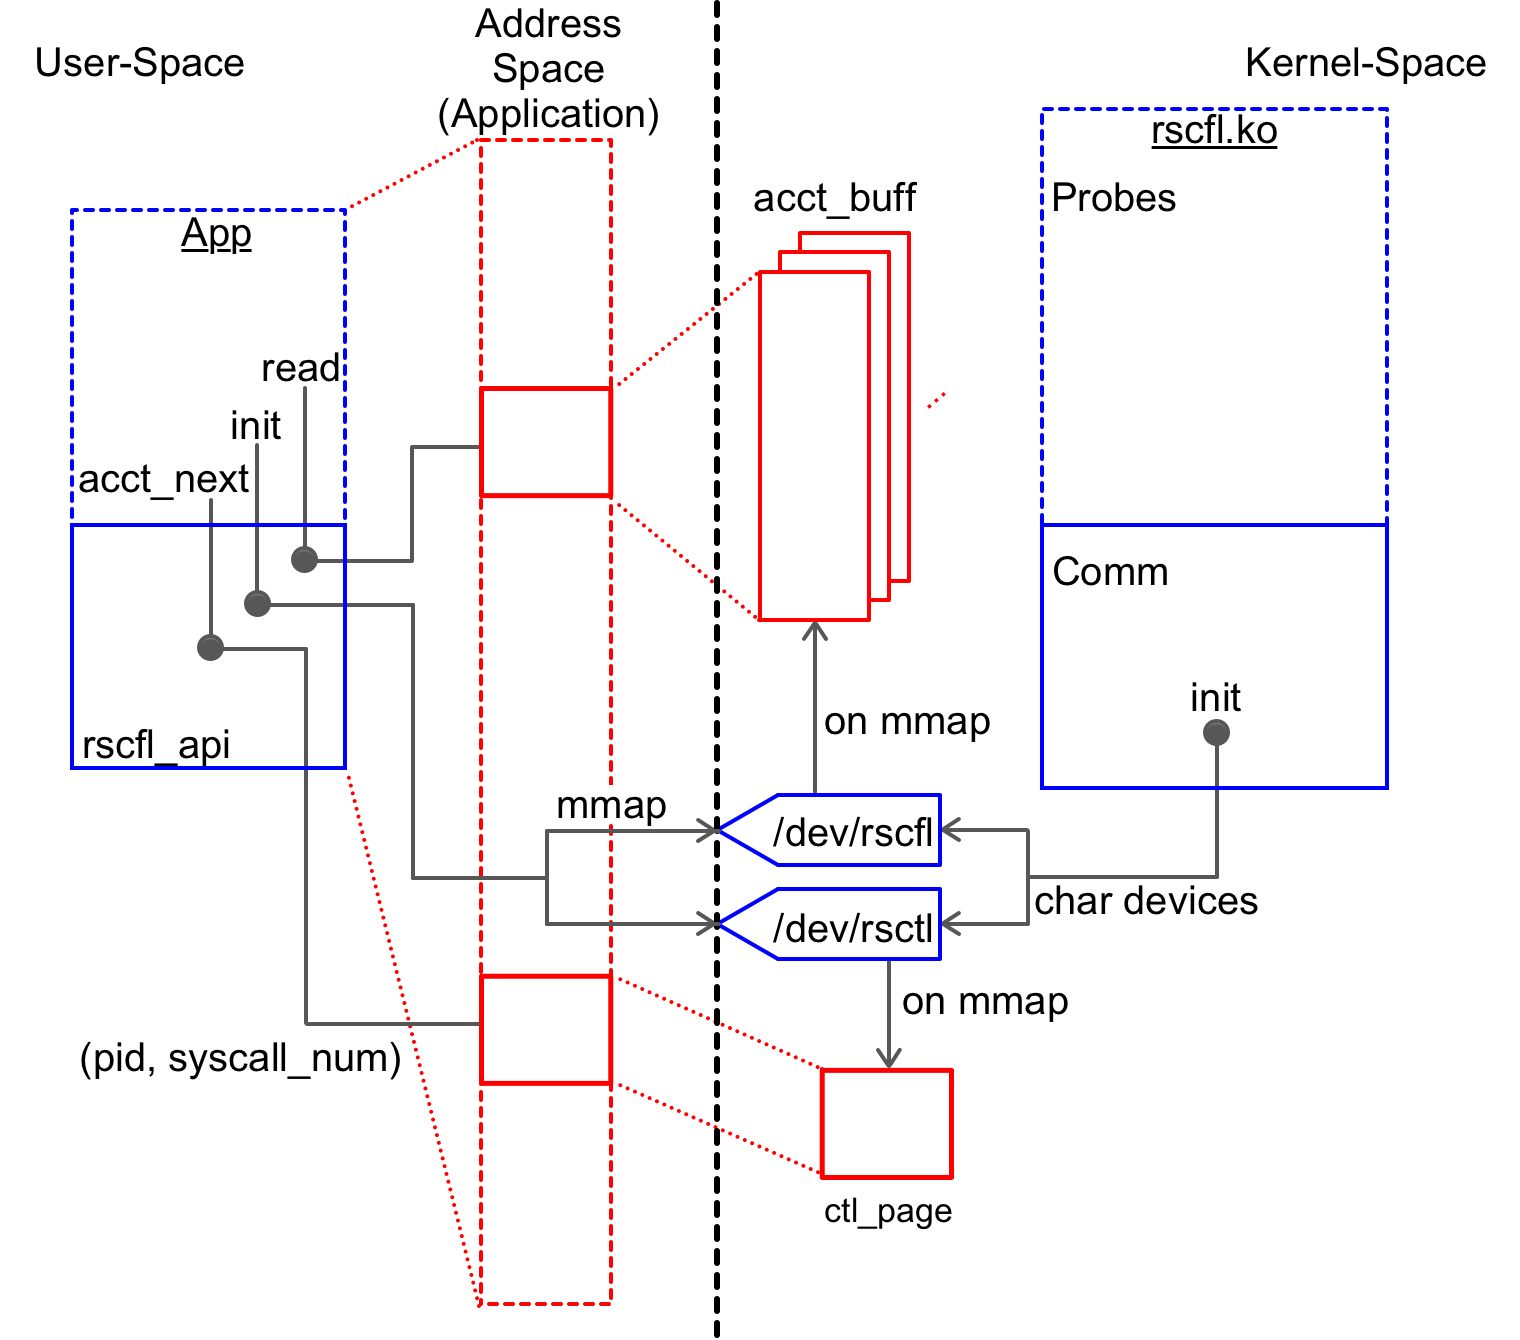
\includegraphics[width=\columnwidth]{sys_design}
    \caption{Primary user-space/kernel-space interactions detailed. Resource accounting data is requested by applications for specific system calls and is then available for reading (zero-copy) from kernel buffer regions mmap-ed into the current address space. }
    \label{fig:design}
\end{figure}

\pname{ }, unlike existing approaches to performance measurement, reports the asynchronous cost of performing a system call.
For instance the true cost of performing a write is made up of both the cost of the synchronous part of the system call, and the latent cost of syncing the data to disk.
This absolute cost of performing a write that flushes buffers, or performing a sync will be higher than a write that is immediately buffered.
We argue that without reporting this amortized, asynchronous cost, performance monitoring APIs give an incomplete representation of system consumption.

\pname{ } performs accounting for asynchronous kernel effects by observing that Linux provides a number of abstractions for performing asynchronous work: \emph{timers}, \emph{tasklets}, and \emph{interrupts}.
\lnote{How have we implemented this?}

\pname{ } is primarily a kernel-accounting framework, so whilst further coalescing, and buffering may be present in hardware, we do not account for this.

% Async / Sync tracing (multiple layers, kworkers etc).

Call granularity tracing.

Trace-point idenfitication - CScope, call site vs function.

Moving from ST to KProbes (more dynamic).

\subsection{User space API}
Interface definition.

Discussion around automatically adding this (compiler).	

\section{Prototype Implementation and Evaluation}
Manual, cross-layer approach while we implement the compiler based approach
Implemented purely to show that runtime overhead is small enough to not be a major issue
Use coarse-grained approach, using existing toold (kprobes, interrupt driven etc)
Cross-layer capture
[Implentation details and results]

Describe use case (lighttpd).\newline
End-to-end example of use of resourceful. Show this is useful. `We show how this
is useful.'

Overhead evaluation.\newline
Space / time overhead. Mem. consumed. Time o/h of various workloads.

Latency and throughput degradation.\newline
For instrumented lighttpd. For something else running at the same time.


\section{Related Work}
Existing tracing / profiling systems. (Maybe a chart outlining differences).

FTrace, SystemTap (raw) / DTrace, Perf.

Existing use of tracing for dependability.\newline
Root-cause analysis. Debugging. Performance monitoring - how do we compare to
top?

\section{Conclusion}
Open Challenges:\\
Accuracy and preciseness,
Low instrumentation overhead,
Generalisability,
Declarative Expressiveness

\section{Acknowledgments}

We thank everyone, and especially those who have funded our work.

{\footnotesize \bibliographystyle{acm}
\bibliography{hotdep}}



\end{document}
